\documentclass[14pt, russian]{matmex-diploma-custom}

\input{preamble.tex}

\begin{document}
\input{title.tex}
\maketitle

% Добавьте эту строку для генерации оглавления:
\tableofcontents

% Теперь идут сами разделы:
% !TeX spellcheck = ru_RU
% !TEX root = vkr.tex

\section*{Введение}
\thispagestyle{withCompileDate}

В современном мире информационные технологии и вычислительные системы стремительно развиваются. Вычислительная мощность устройств увеличивается с каждым годом, а их размеры уменьшаются.

В рамках работы рассматривается задача определения позиций (трекинг) объектов по расстояниям распределенных сенсоров в условиях помех. На фоне технологического прогресса решение такой задачи существенно усложнилось, поскольку объекты наблюдения стали более сложными, быстрыми и непредсказуемыми.

Традиционным подходом к решению задачи является централизованное решение, при котором выделяется единый вычислительный узел, собирающий данные с сенсоров, выполняющий необходимые вычисления и формирующий управляющее воздействие. У такого подхода можно выделить три слабых места:
\begin{itemize}
    \item время на передачу данных от сенсоров до вычислителя;
    \item обработка данных и вычисления;
    \item время на передачу управляющего воздействия от вычислителя обратно к сенсорам.
\end{itemize}
Современные технологии позволяют перейти от этого метода к более новому и эффективному мультиагентному подходу, который устраняет ключевые недостатки централизованной архитектуры, такие как единая точка отказа и ограниченная масштабируемость. В его рамках сенсоры сами выступают в роли вычислительных узлов: они могут самостоятельно определять траекторию объектов, используя как собственные измерения расстояний до целей, так и данные, полученные от соседних сенсоров. Такой подход повышает устойчивость системы, снижает задержки при обработке информации и позволяет более гибко адаптироваться к изменениям в окружающей среде.

К сожалению, на сегодняшний день не существует единой универсальной системы с набором уже реализованных мультиагентных подходов, которая позволяла бы быстро и эффективно протестировать новый мультиагентный алгоритм трекинга и корректно сравнить его с существующими аналогами в одинаковых условиях. Это существенно замедляет проведение исследований, так как исследователям приходится тратить значительное время на самостоятельную реализацию других алгоритмов при отсутствии открытого исходного кода, а также на подготовку симуляций и настройку экспериментальной среды.

% !TeX spellcheck = ru_RU
% !TEX root = vkr.tex

\section{Постановка задачи}
\label{sec:task}
Целью данной дипломной работы является разработать систему для анализа мультиагентных алгоритмов для определения позиций объектов в условиях возмущений и помех не обладающих традиционным статистическим предположениями. Для достижения этой цели были сформулированы следующие задачи.
\begin{enumerate}
    \item Провести обзор существующих систем для анализа мультиагентных алгоритмов.
    \item Сформулировать требования к разрабатываемой системе.
    \item Разработать архитектуру системы на основе требовани.
    \item Реализовать систему.
    \item Интегрировать в систему существующие мультиагентные алгоритмы в качестве эталонов для сравнения и провести их валидацию.
\end{enumerate}
% !TeX spellcheck = ru_RU
% !TEX root = vkr.tex

\section{Сбор требований}

В результате взаимодействия с членами научной группы, занимающейся
разработкой рассматриваемых алгоритмов, были сформулированы требования
к разрабатываемой системе. Эти требования отражают как особенности
предметной области, так и ограничения существующих инструментов.

\begin{enumerate}
    \item \textbf{Поддержка пользовательских аккаунтов и загрузки алгоритмов.}  
    Система должна обеспечивать возможность создания пользовательских
    аккаунтов, а также предоставлять интерфейс для загрузки и интеграции
    пользовательских алгоритмов. Это необходимо для проведения
    сравнительных исследований различных подходов в единой среде.
    
    \item \textbf{Гибкая настройка параметров симуляции.}  
    Должна быть предусмотрена возможность задания параметров сценария,
    включая количество целей и сенсоров, продолжительность моделирования,
    характер движения целей, а также параметры возмущений и помех.
    Это позволяет исследовать устойчивость алгоритмов в различных условиях.
    
    \item \textbf{Визуализация результатов моделирования.}  
    Система должна предоставлять средства для наглядного отображения
    результатов, включая траектории движения целей и эволюцию
    среднеквадратической ошибки. Визуализация является важным инструментом
    анализа качества алгоритмов.
    
    \item \textbf{Поддержка пакетного запуска экспериментов.}  
    Необходима возможность автоматизированного запуска серии сценариев
    с последующей агрегацией результатов. Это существенно упрощает
    проведение масштабных экспериментальных исследований.
    
    \item \textbf{Поддержка сравнения результатов при различных параметрах.}  
    Система должна обеспечивать средства для сравнения результатов работы
    алгоритмов при различных настройках симуляции, что позволяет выявлять
    зависимости качества работы алгоритмов от всех настраиваемых параметров.
\end{enumerate}

\vspace{0.5em}

Приведенный ниже анализ отражает необходимость в специализированной
системе, ориентированной на проведение воспроизводимых и масштабируемых
экспериментов с мультиагентными алгоритмами трекинга в условиях
возмущений и помех.
% !TeX spellcheck = ru_RU
% !TEX root = vkr.tex

\section{Обзор}
\label{sec:relatedworks}

В данном разделе нужно описать всё, что необходимо для понимания Вашей работы и что придумали не Вы.
В дальнейших разделах нельзя прерывать повествование, например, для рассказа о деталях используемой технологии или архитектуре старой системы, потому что читателю будет трудно отличить Ваш вклад от не Вашего.

Любой обзор пишется с какой-то целью (обосновать актуальность, найти и описать интересные решения, сравнить и выбрать технологии) и по какой-то методике поиска материала (например, поиск N релевантных статей на таких-то сервисах).
Не будет лишним это всё явно описать.

\subsection{Обзор существующих решений}

В настоящее время существует ряд программных средств и библиотек,
предназначенных для моделирования мультиагентных систем и трекинга объектов. Однако большинство из них либо
ориентированы на централизованные методы обработки, либо не учитывают
специфику рассматриваемой задачи — анализ мультиагентных алгоритмов
в условиях возмущений и помех, не обладающих стандартными статистическими
предположениями.

\textbf{MATLAB Sensor Fusion and Tracking Toolbox} предоставляет широкий
набор инструментов для моделирования сенсоров, трекинга объектов и оценки
качества алгоритмов. К его преимуществам относятся развитая экосистема,
наличие готовых реализаций алгоритмов и удобные средства визуализации.
Однако данный инструмент в первую очередь ориентирован на централизованные
подходы к обработке данных. Кроме того, система является закрытой и требует
дорогостоящей лицензии, а интеграция пользовательских мультиагентных
алгоритмов затруднена.

\textbf{Repast (Agent-Based Modeling Toolkit)} представляет собой универсальную
платформу для моделирования мультиагентных систем. К её преимуществам можно
отнести гибкость и возможность описания широкого класса агентных моделей.
Тем не менее, данная платформа в основном применяется в социально-экономических
и биологических задачах и не содержит встроенных средств для моделирования
сенсоров и алгоритмов трекинга. Также стоит отметить, что система в настоящее
время активно не развивается и ограниченно поддерживается.

\textbf{SIMLAN и симуляторы на базе Gazebo} широко используются в задачах
робототехники для моделирования поведения роботов и тестирования алгоритмов
навигации. Их основным преимуществом является высокая степень реалистичности
физической симуляции и развитые средства интеграции с робототехническими
платформами. Однако такие системы ориентированы на детальное моделирование
физической среды и являются избыточными и сложными в настройке для задач
абстрактного анализа алгоритмов трекинга. Кроме того, они не предоставляют
удобных средств для массового сравнительного анализа алгоритмов.

\vspace{0.5em}

Для наглядного сравнения рассмотренных решений приведём таблицу
(табл.~\ref{tab:comparison_existing_systems}).

\begin{table}[h]
    \centering
    \caption{Сравнение существующих решений}
    \label{tab:comparison_existing_systems}
    
    \resizebox{\textwidth}{!}{
    \begin{tabular}{|l|c|c|c|}
    \hline
    \textbf{Характеристика} & \textbf{MATLAB Toolbox} & \textbf{Repast} & \textbf{Gazebo / SIMLAN} \\
    \hline
    Поддержка мультиагентных алгоритмов & $\pm$ & + & $\pm$ \\
    \hline
    Встроенные модели сенсоров & + & - & + \\
    \hline
    Инструменты трекинга & + & - & $\pm$ \\
    \hline
    Простота интеграции своих алгоритмов & - & + & - \\
    \hline
    Пакетные эксперименты и сравнение & $\pm$ & - & - \\
    \hline
    Визуализация результатов & + & $\pm$ & + \\
    \hline
    Ориентация на распределённые алгоритмы & - & $\pm$ & $\pm$ \\
    \hline
    Нестандартные статистические условия & - & - & - \\
    \hline
    \end{tabular}
    }
    \end{table}

\vspace{0.5em}

\textbf{Вывод.}
Проведённый анализ показал, что существующие решения либо ориентированы
на централизованные методы обработки данных, либо не предоставляют
необходимых инструментов для моделирования сенсорных систем и трекинга,
либо избыточны для рассматриваемой задачи. Кроме того, ни одна из систем
не поддерживает в полной мере проведение экспериментов в условиях
нестандартных статистических предположений.

Таким образом, существует необходимость в разработке специализированной
системы, позволяющей интегрировать пользовательские мультиагентные алгоритмы,
гибко задавать параметры симуляции и проводить их сравнительный анализ
в условиях возмущений и помех произвольной природы.


\section{Архитектура}
\subsection{Структура системы}

На основе требований, сформулированных в разделе сбора требований,
была разработана модульная архитектура системы, обеспечивающая
гибкость, расширяемость и возможность проведения воспроизводимых
экспериментов.

Общая структура системы представлена на (рис.~\ref{fig:architecture}).

\begin{figure}[h!]
    \centering
    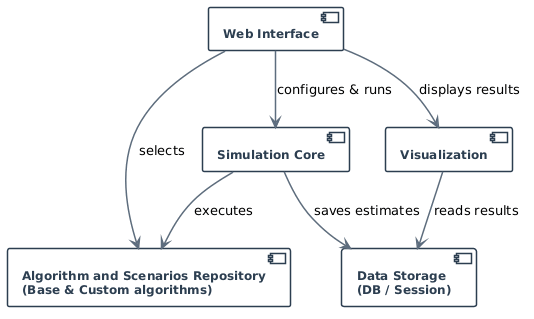
\includegraphics[width=0.9\textwidth]{arch.png}
    \caption{Архитектура системы моделирования}
    \label{fig:architecture}
\end{figure}

Архитектура системы включает следующие основные компоненты:

\begin{itemize}
    \item \textbf{Web Interface (веб-интерфейс).}  
    Обеспечивает взаимодействие пользователя с системой. Через данный
    компонент осуществляется настройка параметров симуляции, выбор
    алгоритмов, запуск экспериментов и просмотр результатов.

    \item \textbf{Simulation Core (ядро моделирования).}  
    Центральный компонент системы, отвечающий за выполнение симуляции,
    генерацию движения целей и обработку наблюдений с учётом шумов.

    \item \textbf{Algorithm Repository (репозиторий алгоритмов).}  
    Содержит базовые и пользовательские алгоритмы и предоставляет
    унифицированный интерфейс для их выполнения.

    \item \textbf{Data Storage (хранилище данных).}  
    Отвечает за сохранение результатов моделирования, параметров
    экспериментов и промежуточных вычислений.

    \item \textbf{Visualization (подсистема визуализации).}  
    Обеспечивает отображение результатов в виде графиков траекторий
    и кривых ошибок.
\end{itemize}

Взаимодействие компонентов (рис.~\ref{fig:architecture}) организовано
следующим образом: пользователь через веб-интерфейс задаёт параметры
симуляции и выбирает алгоритмы, после чего управление передаётся в ядро
моделирования. Ядро обращается к репозиторию алгоритмов, сохраняет
результаты в хранилище и передаёт их в подсистему визуализации.

Таким образом, архитектура удовлетворяет требованиям:
поддержки пользовательских алгоритмов, гибкой настройки,
визуализации и пакетной обработки экспериментов.

\subsection{Пользовательский сценарий}

Типовой пользовательский сценарий работы с системой представлен
на (рис.~\ref{fig:usecase}).

\begin{figure}[h!]
    \centering
    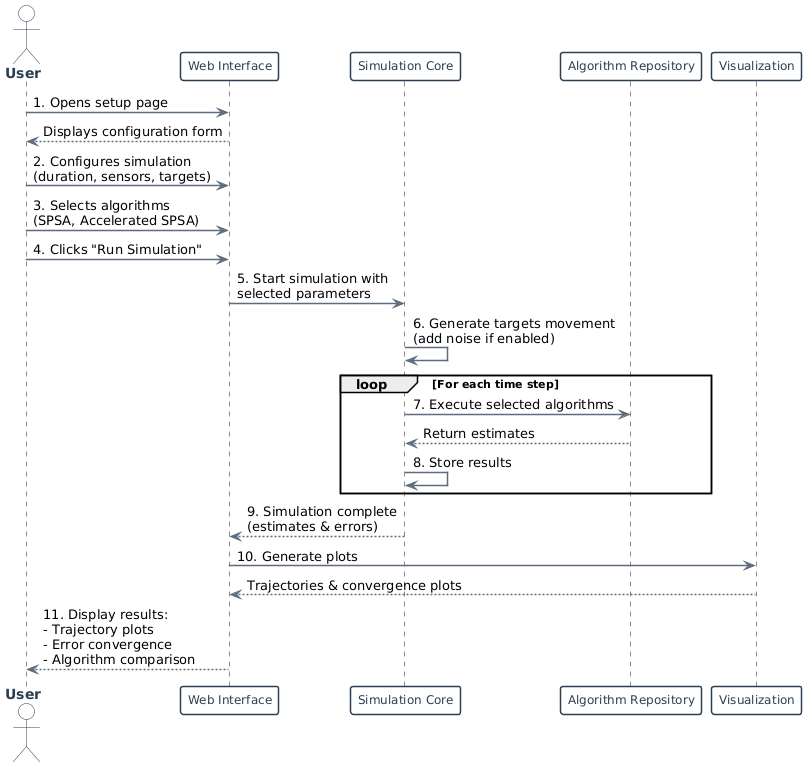
\includegraphics[width=0.95\textwidth]{use_case.png}
    \caption{Сценарий взаимодействия пользователя с системой}
    \label{fig:usecase}
\end{figure}

Сценарий работы пользователя включает следующие этапы:

\begin{enumerate}
    \item \textbf{Открытие страницы настройки.}  
    Пользователь переходит в веб-интерфейс и получает доступ к форме
    конфигурации.

    \item \textbf{Задание параметров симуляции.}  
    Пользователь задаёт длительность моделирования, количество целей и
    сенсоров, а также параметры шумов.

    \item \textbf{Выбор алгоритмов.}  
    Из репозитория выбираются алгоритмы для сравнения.

    \item \textbf{Запуск симуляции.}  
    Пользователь инициирует выполнение эксперимента.

    \item \textbf{Выполнение моделирования.}  
    Ядро моделирования выполняет расчёты, на каждом шаге времени
    вызывая выбранные алгоритмы.

    \item \textbf{Получение результатов.}  
    После завершения моделирования результаты передаются в систему
    визуализации.

    \item \textbf{Анализ результатов.}  
    Пользователь анализирует траектории, ошибки и сравнивает алгоритмы.
\end{enumerate}

Дополнительно система поддерживает пакетный режим, позволяющий
запускать серию экспериментов с последующим агрегированием результатов.

Таким образом, пользовательский сценарий (рис.~\ref{fig:usecase})
обеспечивает полный цикл работы с системой и соответствует
сформулированным требованиям.
% !TeX spellcheck = ru_RU
% !TEX root = vkr.tex

\section{Особенности реализации}

\subsection{Используемый стек технологий}
\subsection{Симуляция}
\subsection{Реализованные алгоритмы}

В рамках работы в систему интегрированы следующие мультиагентные алгоритмы определения позиций объектов.

\subsubsection{Алгоритм на основе SPSA}


\[
\left\{
\begin{aligned}
  &\mathbf{x}_{2k}^i = \hat{\boldsymbol{\theta}}_{2k-2}^i + \beta_k^+ \boldsymbol{\Delta}_k^i, \\[0.5em]
  &\mathbf{x}_{2k-1}^i = \hat{\boldsymbol{\theta}}_{2k-2}^i - \beta_k^- \boldsymbol{\Delta}_k^i \\[0.5em]
  &\hat{\boldsymbol{\theta}}_{2k-1}^i = \hat{\boldsymbol{\theta}}_{2k-2}^i, \\[0.5em]
  &\hat{\boldsymbol{\theta}}_{2k}^i = \hat{\boldsymbol{\theta}}_{2k-1}^i - \alpha \left( \frac{y_{2k}^i - y_{2k-1}^i}{\beta_k} \mathbf{K}_k^i(\boldsymbol{\Delta}_k^i) \right. \\[0.5em]
  &\qquad \left. {} + \gamma \sum_{j \in \mathcal{N}_{2k-1}^i} b_{2k-1}^{i,j} (\tilde{\theta}_{2k-1}^{i,j} - \hat{\theta}_{2k-1}^i) \right)
\end{aligned}
\right.
\]


\paragraph{Пояснение основных шагов.}

\begin{enumerate}
    \item \textbf{Формирование текущей оценки.}  
    Агент использует предыдущее состояние $\hat{\theta}_{2k-2}^i$ как базовую точку $x_k^i$.

    \item \textbf{SPSA-возмущение.}  
    Генерируется случайный вектор $\Delta_k^i \in \{\pm 1\}^d$ и формируются две точки:
    $x_{2k}^i$ и $x_{2k-1}^i$.

    \item \textbf{Оценка градиента.}  
    Производится симметричная разностная аппроксимация:
    \[
    \frac{y_{2k}^i - y_{2k-1}^i}{\beta_k}\Delta_k^i.
    \]

    \item \textbf{Консенсусный шаг.}  
    Добавляется вклад соседей через граф взаимодействия:
    \[
    \sum_{j \in \mathcal{N}_i} b^{i,j} (\hat{\theta}^j - \hat{\theta}^i).
    \]

    \item \textbf{Обновление параметров.}  
    Выполняется градиентный шаг:
    \[
    \hat{\theta}_{2k}^i = \hat{\theta}_{2k-1}^i - \alpha g_k^i.
    \]
\end{enumerate}

\subsubsection{Ускоренный алгоритм на основе SPSA + Консенсус}


\[
\left\{
\begin{aligned}
  &\bar{\mathbf{x}}_k = \dfrac{1}{\gamma_{k-1} + \alpha_k(\mu - \eta)} \Big( \alpha_k \gamma_{k-1} \bar{\mathbf{z}}_{k-1} + \gamma_k \bar{\boldsymbol{\theta}}_{2k-1} \Big), \\[0.8em]
  &\bar{\mathbf{x}}_{2k} = \bar{\mathbf{x}}_k + \beta_k^+ \bar{\boldsymbol{\Delta}}_k, \quad
  \bar{\mathbf{x}}_{2k-1} = \bar{\mathbf{x}}_k - \beta_k^- \bar{\boldsymbol{\Delta}}_k, \\[0.8em]
  &\bar{\mathbf{g}}_k = \left( \dfrac{\bar{\mathbf{y}}_{2k} - \bar{\mathbf{y}}_{2k-1}}{\beta_k} \otimes \mathbf{I}_d \right) \bar{\boldsymbol{\Delta}}_k + \omega \left( \bar{\mathcal{L}}_{2k-1} \otimes E_n \right) \bar{\mathbf{x}}_k, \\[0.8em]
  &\bar{\boldsymbol{\theta}}_{2k} = \bar{\mathbf{x}}_k - h \bar{\mathbf{g}}_k, \\[0.5em]
  &\bar{\boldsymbol{\theta}}_{2k+1} = \bar{\boldsymbol{\theta}}_{2k}, \\[0.5em]
  &\bar{\mathbf{z}}_k = \dfrac{(1 - \alpha_k) \gamma_{k-1} \bar{\mathbf{z}}_{k-1} + \alpha_k (\mu - \eta) \bar{\mathbf{x}}_k - \alpha_k \bar{\mathbf{g}}_k}{\gamma_k}
\end{aligned}
\right.
\]

\paragraph{Пояснение основных шагов.}

\begin{enumerate}
    \item \textbf{Формирование точки зондирования $\tilde{x}_k$.}  
    Это взвешенная комбинация предыдущего состояния $\theta$ и вспомогательной переменной $z_k$.  
    Она играет роль ``ускоренной'' точки, аналогично методам Нестерова.

    \item \textbf{Случайное возмущение (SPSA).}  
    Генерируется случайный вектор $\Delta_k$ (обычно Бернулли $\pm 1$).  
    Затем вычисляются две точки:
    \[
    x_{2k},\quad x_{2k-1}
    \]
    что позволяет оценить градиент без явных производных.

    \item \textbf{Оценка градиента.}  
    Градиент аппроксимируется как
    \[
    g_k \approx \frac{f(x+\beta\Delta) - f(x-\beta\Delta)}{2\beta}\Delta,
    \]
    с добавлением консенсусного члена $\omega L x_k$, учитывающего взаимодействие агентов.

    \item \textbf{Шаг спуска.}  
    Выполняется обновление:
    \[
    \theta_{2k} = \tilde{x}_k - h g_k,
    \]
    где $h$ — шаг обучения.

    \item \textbf{Ускорение (переменная $z_k$).}  
    Вводится вспомогательная последовательность $z_k$, которая аккумулирует информацию о предыдущих итерациях и обеспечивает ускоренную сходимость.

    \item \textbf{Обновление параметров ускорения.}  
    Параметры $\alpha_k$ и $\gamma_k$ обновляются рекурсивно:
    \[
    \gamma_k = (1-\alpha_k)\gamma_{k-1} + \alpha_k(\mu - \eta),
    \]
    что задаёт динамику ускорения.
\end{enumerate}
\section*{Заключение}

В ходе выполнения работы были получены следующие результаты.

\begin{itemize}
    \item Проведён обзор существующих инструментов для моделирования и анализа мультиагентных систем, включая MATLAB Sensor Fusion and Tracking Toolbox, Repast (Agent-Based Modeling Toolkit) и SIMLAN, с точки зрения их применимости к задачам трекинга.
    
    \item Собраны и систематизированы требования от членов научной группы, разрабатывающих современные мультиагентные алгоритмы трекинга. Требования структурированы по ключевым группам: генерация сценариев (сенсоры, объекты, помехи), поддержка алгоритмов (базовые реализации и возможность интеграции пользовательских), а также средства сравнительного анализа (визуализация ошибок и траекторий).
    
    \item Спроектирована модульная архитектура системы, обеспечивающая разделение компонентов симуляции, выполнения алгоритмов и визуализации. Разработан пользовательский сценарий, в рамках которого исследователь задаёт параметры эксперимента, запускает вычислительный конвейер и получает наглядное сравнение эффективности алгоритмов.
    
    \item Реализована программная система в виде веб-приложения на основе фреймворка Django, обеспечивающая доступ к функциональности через удобный пользовательский интерфейс.
    
    \item Интегрированы эталонные мультиагентные алгоритмы трекинга: алгоритм на основе SPSA, его ускоренная версия и распределённый фильтр Калмана, используемые в качестве базовой линии для сравнения новых алгоритмов.
    
    \item Результаты работы представлены на XXVII конференции молодых учёных «Навигация и управление движением», а также опубликованы в журнале IEEE Transactions on Automatic Control.
\end{itemize}

\noindent Исходный код разработанной системы: \textit{[добавьте ссылку на репозиторий]}.

\setmonofont{CMU Typewriter Text}
\bibliographystyle{ugost2008ls}
\bibliography{vkr}

\end{document}